\cleardoublepage
\singlespacing
\chapter{Reconfigurable Atomic Service for Component Objects}
\label{c:rasco}
\doublespacing\nointerlineskip

This chapter presents the Reconfigurable Atomic Service for Component Objects,
RASCO in short. First, the profile framework is described in section~\ref{s:pf}.
Section~\ref{s:ss} describes a new redundancy configuration model called Strips
to track and handle redundant WuObjects dynamically. After that section~\ref{s:dfd}, ~\ref{s:fr} and ~\ref{s:reconfig} presents the distributed algorithm used to
solve the problem. %#############The models and algorithms are tested extensively on various benchmarks, described in section~\ref{s:benchmarks}, and the results are discussed and compared with existing fault tolerant system models in section~\ref{s:results}##############

\section{Profile Framework}
\label{s:pf}

In this work, we build upon WuKong, a loosely-coupled component based
architecture for M2M systems. WuKong uses profile
framework to enable the handling of physical resources on heterogeneous sensor
nodes, and for higher abstractions of software component capabilities. As
future M2M systems could consist of many heterogeneous sensor nodes and
actuator nodes, two main concepts in profile framework, namely WuClass and
WuObject, was introduced to allow WuKong to track, and manage physical
resources in the network.~\cite{Reijers} However WuKong has no support for
fault tolerance. We proposed a solution to track, manage and maintain
consistency among nodes based on concepts of WuClasses and WuObjects from
profile framework. Nodes duplicate WuObjects, such as WuClass ids but not
their respective ports on their respective hosts, and link information. Among
the hosts that have the same WuObjects, only one is active and is the primary
service provider in the eyes of other services and clients.

\section{Strips} % good name?
\label{s:ss}

\begin{figure}[h!]
\caption{An example network with several strips}
\label{fig:strips-network}
\centering
    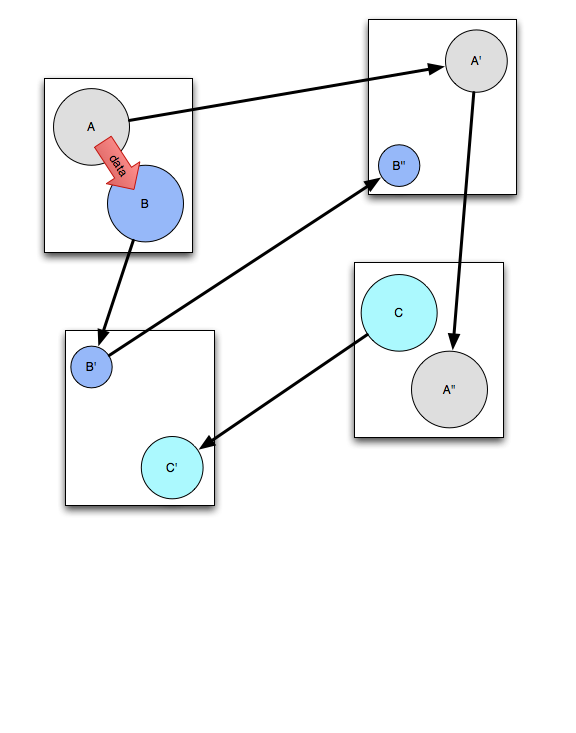
\includegraphics[width=\linewidth]{figures/strips-network}
\end{figure}

This work proposed an algorithm that uses strips. Strips are a sequence of
WuObjects on different nodes where the node holding the first WuObject is
active in the system while the rest are backups. The order of a strip is
typically determined by the system that deploys the application. Strips
consists of members which are chained together in series to the next that when
one member failed, the next one will take over, except the last one. For
example, for a strip constructed like this $\rightarrow 1-2-3-4-5$, when
3 failed 4 will take over the place of 3 and shift all the objects after it
forward, and the new chain will look like this: $\rightarrow 1-2-4-5$. Now if
1 failed, 2 will take over and members after 2 (including 2) will shift one
position forward that would result in $\rightarrow 2-4-5$. When a backup
becomes the head of the strip, it will become active in the system.

In a heterogeneous network, each host could carry more than one WuObjects.
Since each strip represents a specific component in the application, there will
typically be many of these strips present in the network where each of them
could crisscross with one and others. So it is typical that a node could be
carrying inactive WuObjects and active WuObjects at the same time.

A node stores membership information of the strips where it is a member of. As
later sections will also introduce to the heartbeat protocols that each node will
be monitoring some other nodes, each node will also store the membership
information of the strips of the nodes it is monitoring. Each stripe is stored
as a list with membership address information in the same order as the order of the
strips so for example, the current head of the strip is the first element of
the list. Nodes use the information stored to track and notify the nodes for
any changes in the strips.

Figure~\ref{fig:strips-network} illustrates a network with many strips as
strips crisscross and layout in the network. Each block represents a host, and
each circle is a WuObject. Notice that only the head (ones with no arrows
pointing at) of the strip is active and will have data flow through them as
represented by a thick arrow. The name of the component represents the type of
the component, and duplications have the same name as the component but with an
apostrophe next to it. As shown in the figure~\ref{fig:strips-network}, each
strip could crisscoss and could have duplication residing with another component
within the same host.

\section{Decentralized Failure Detection}
\label{s:dfd}

The system assumes a fully connected heterogeneous network with sensors and
actuators where each node in the network could host multiple components. This
work uses heartbeat technique, a popular technique widely used to detect
failures in high-availability distributed systems. Each node would send
a heartbeat message to its detector periodically in a fixed interval
until it's unable to send messages anymore. Each node is therefore suspected
dead when it stops sending messages after a period of time.

There are many related work on heartbeat protocols to ensure high-availability
whether it uses star topology, or a ring topology; the main purpose for
a heartbeat protocol is to detect failure within a network as fast as possible.
Our work assumed a ring topology heartbeat protocol such that a node A would
send heartbeat to node B and so on, but the last node would send heartbeat back
to node A.

However, the heartbeat protocol used in the network is not directly related to
the ordering of the strips. The heartbeat protocol is a layer below the strips
as a support for network fault detection, the algorithm above will take
advantage of the given information from the layer below to recover the system.

One of the reasons this is good for the system is extensibility and
separation of concerns, by excluding both domains into separate layers each
layer could optimize on its own record without being binded by another layer
which might hinder each other. The separation of concerns would make each layer
modular and be able to switch and plug in for a different algorithms that might
result in a better performance for a particular deployment. Besides, because
every node could carry more than one WuObject, and the distribution of the
WuObjects might not always be ideal and evenly spread out to the network,
heartbeat protocol designed around current strip assignments will not
be able to cover the whole network or to be optimized in communication overhead.

\section{Failure Recovery}
\label{s:fr}

When a failure is detected, there are two tasks that the system will have to do
to recover from failures. First it has to make sure all members that carries
the strips in the failure nodes will have consistent view of the strips.
Second, it would need to propagate the changes to reconfigure other parts of
the system that depend on the locations of the heads of the affected strips in
order to function. The work built on a stateless system as defined by WuKong
middleware with FBP applications where none of the services need to store any
states or to remember any history. For example, WuKong applications don't have
services that require to store past values of some variables. Therefore strips
members (except the head) with inactive WuObjects are not the same replication
as defined in other related work, but simply as backups that will take over
when the active WuObject failed.

% should state stateless distributed system to enable no replication in the
% sense of other related work

% should also state how it is stateless, and how it is different from other
% distributed systems

\subsection{Consistency among strip members}

Typically several strips would be cut off in the event of failure, and if the
failed node carries some active WuObjects from some strips, the system would
not able to continue to function. RASCO will attempt to recover by letting the
detector of the failure to initiate the recovery algorithms.
Since the detector will be responsible for recoverying for the failed node,
every node needs to have membership knowledge of the strips from the nodes it
is monitoring. For example, if node A is monitoring node B, A would know the
members of all strips in node B in addition to its local strips. Strips only
specifies the order of recovery, it is not correlated with the network
structure for the fault detection, in other words, a strip with A and B doesn't
mean B is monitoring A, as B could be monitored by C which depends on the
structure of heartbeat protocol layer.
In the initial algorithm, the detector node will prepare a update message to
inform all members of the strips with which the failed node is associated with.
Assuming that every node that monitors other node will have knowledge of the
strips that it contains and the members that the strips pertain. The node would
send out a marker multicast first to confirm the nodes which are still
functioning, and once all acknowledges have been received, it will proceed to
send the update message to update their local knowledge of the strips to reach
a consensus. The ordering of the messages wouldn't matter since the end state
of any failure sequence for any strip would be the same. For example, given
a strip of three members $\rightarrow 1-2-3$, if the updated failure sequence
is given in any permutation by $[1, 2]$ or $[2, 1]$, the end results would be
the same $\rightarrow 3$ since the remaining members from those two failure
sequence is the same and the relative order of the members would stay the same.
\begin{comment}
Let's assume there is a pair of failure patterns with the same members but
different orders that would do update operations on the same strip but would
leave the strip in different results. If that's true, then by building back the
strips from the result in the order of update operations would result in
a different starting state, that implies the strips have different members or
member orders to start with, a contradiction.
\end{comment}
Therefore there is no need for extra communication overhead to maintain
ordering to gaurantee level of consistency between members since they will all
come to the same conclusion given each receiver receive the same messages. The
overhead are messages required to update each member's internal membership
information.

\subsection{Reconfiguration}
\label{s:reconfig}

\begin{figure}[h!]
\caption{A reconfiguration of a Network}
\label{fig:reconfig-network}
\centering
    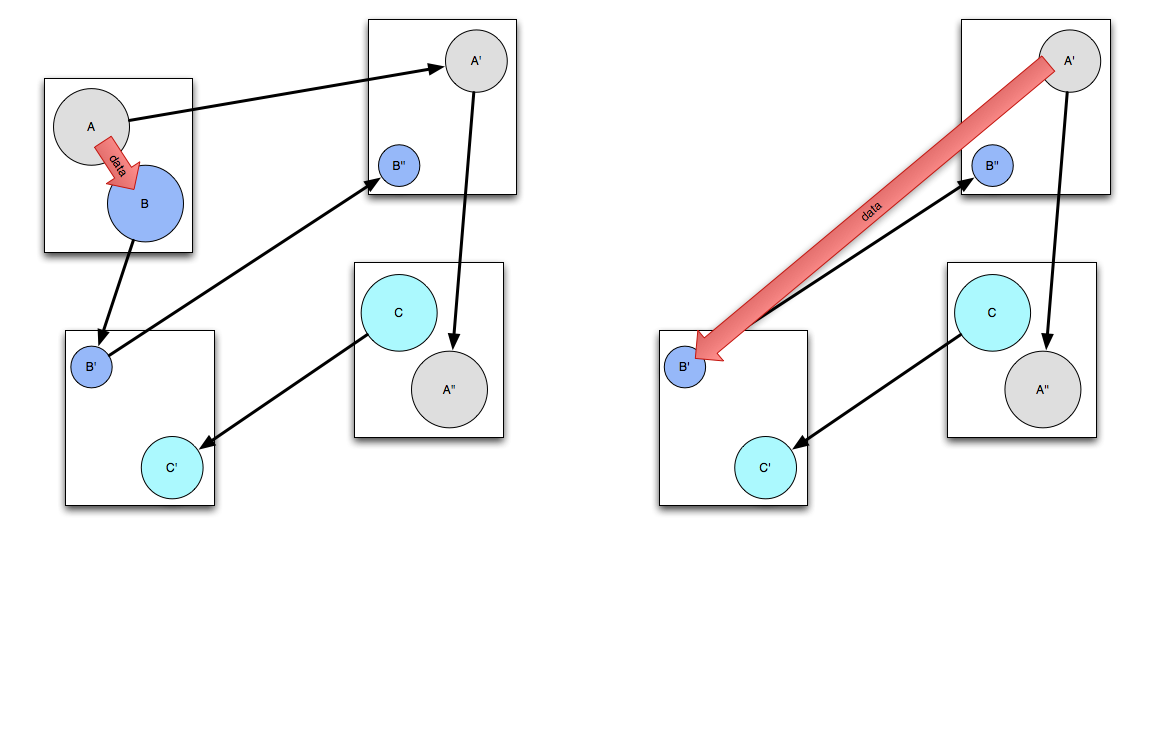
\includegraphics[width=\linewidth]{figures/reconfig-network}
\end{figure}

Even though consensus of the new configuration for each affected strip has been
reached, some nodes with component that acts as a client to another component
for data or the reverse would also have to have consensus on the updated
primary holder of each affected component. And the node that is monitoring the
node monitored by the dead node would also need to update on its knowledge of
its monitored node in order to recover the next possible failure.

RASCO will initiate a reconfiguration service to reconfigure the network to adapt
to the new strip configurations. Reconfiguration service is implemented by
a distributed algorithm which is inititated by the detected nodes. First the
initiator node would have to identify the components that are reading/writing
data with the components carried by the dead host. This would be done by
requesting the link information between components at the higher level provided
by the application. Then each member of the strips of the connected components
would be updated with the information about the change in the host of the
failed components with a \emph{reconfig} message containing the change in the
location of the specific WuObjects. Right after receiving the \emph{reconfig}
message, if the connected nodes whose WuObjects are pushing data to the
WuObjects on the failed nodes, they will force to initiate a data push to
update and bring the recovered nodes up to date, and vice versa, so the nodes
whose WuObjects are receiving data from the failed nodes will initiate a data
pull after receiving the \emph{reconfig} message.

As shown in figure~\ref{fig:reconfig-network}, the network on the right has
a node failed that bring both current heads of strips A, and B down. As shown
on the right, after recovery, the nodes that have the active WuObjects
connecting to each new heads in both strips A and B both will be updated on the
current location of the heads of both strips. Because the bottom left node
contains the new head of strip B and is connected to strip A, therefore it will
be updated on the location of the new head of strip B, and vice versa.

Reconfiguration service has message complexity of $O(m)$ where m is the
number of strips where its components are linked to the failed components.

\begin{comment} % temporary
\section{Benchmarks}
\label{s:benchmarks}

% here states that we deployed on wireless sensor platform for proving that it
% works for the most resource limited distributed platform
\subsection{Experimental Result}

The performance of the fault tolerance system is evaluated with the metrics listed below:
\begin{enumerate}
\item Correctness, whether the system is configured to do what the mapping result specifies, including the heartbeats, heartbeat periods, recovery chains, application links.
\item Communication overhead used for heartbeats
\item Communication overhead for failure recovery
\item Failure detection success rate
\item Fault recovery success rate
\item The average time to recover from the time of failure
\item The average number of messages used to recover the system
\end{enumerate}
\end{comment} % temporarily

\section{Evaluation}

In order to evaluate the performance of the fault tolerant system on RASCO and Strips, application shown in Figure~\ref{fid:application} will be deployed through WuKong. First we describe the hardware platform that will be hosting the Strips, then we describe the experimental setup for the deployment. Lastly, we present the results with discussion.

\subsection{Hardware Platform}

\begin{figure}[h!]
\caption{An WuDevice}
\label{fig:wudevice}
\centering
    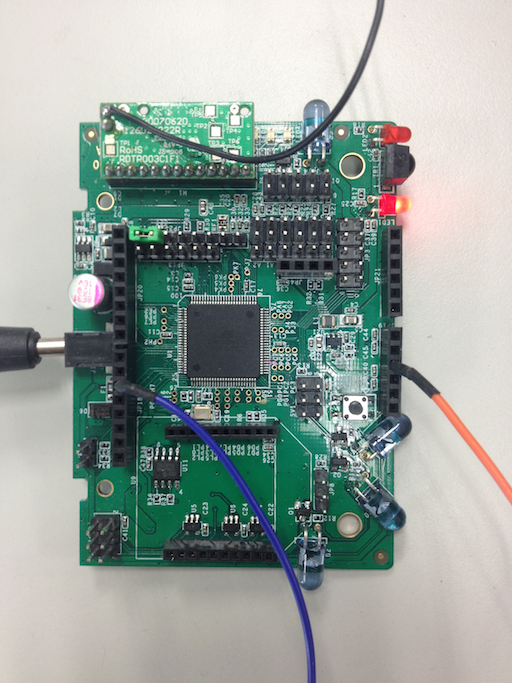
\includegraphics[width=\linewidth]{figures/wudevice}
\end{figure}

All boards are equipped with an Atmel ATmega1280-16AU 8-bit microcontroller with 4K of EEPROM and 64k of flash. The boards hardware design is based upon Arduino hardware referenced design, in addition, every board has wires for mounting multiple wireless protocol adapters such as ZWave, ZigBee. In the following experiments, every board is only equipped with a ZWave adapter, and only communicating through ZWave. 

Every board is also pre-installed with a modified version of NanoVM (ref here) called “NanoKong” that supports all the basic WuKong framework protocols including the new additions from the work in the previous chapter.

A PC with wireless access is dedicated for hosting the WuKong Master software which is responsible for managing WuKong applications for the whole system and serves as a mean to present an interface to the users.

Three boards will be used in the experiments below. One of them is equipped with a light sensor that returns a byte indicating the light level around the sensor. The rest are equipped with a relay which each controls the power supply of a lamp.

An additional board with the same hardware specification is used as a gateway between the Master and the sensor network.

\subsection{Experimental Setup}

% we could do it today
Three WuDevices are deployed in a room where two of them are connected to a 

%Describe limits: 
%1. Fully connected network

In this experiment, an application shown in figure 1 above will be deployed with a fault tolerance user policy shown in the figure 2 upon the hardware setup described in the previous section three times to evaluate its performance.

The application requires a light sensor and a light actuator. The light actuator will turn on the light if the sensed light value is below a threshold specified from the numeric controller. Numeric controller is fixed on a value of 200. The light value takes a byte ranging from 0 to 255. The comparison is done with a virtual component Threshold in native implementation.

We will simulate a node failure by unplugging the power supply of the active light sensor node on all tries.

\subsubsection{Heartbeat Protocols}

\subsubsection{Strips}

\section{Results}
\label{s:results}

